% vim: set spelllang=fr foldmethod=marker:
\section{Problématiques liées aux \rcs}

De par leurs ressources faibles, leur dispersion dans un environnement parfois hostile, leurs communications sans fil, et les différentes missions qui leur sont confiées, les \rcsfs introduisent une multitude de problématiques que l'on ne retrouve pas ou peu dans d'autres types de réseaux.
Nous introduisons ici celles qui sont indispensables à la compréhension des travaux de cette thèse.

    \subsection{Gestion des ressources et performances}
%{{{1
Les évolutions technologiques des dernières décennies n'ont de cesse de rendre les ordinateurs plus performants, plus compacts, plus rapides dans le traitement des données.
Elles ont rendu possible, à force de miniaturisation et de réduction des couts, la création et le déploiement des \rcsfs, mais ceux-ci restent soumis à des contraintes en ressources très fortes par rapport aux stations de travail «classiques» tel que les ordinateurs personnels (y compris portables).

        \subsubsection{Des algorithmes à adapter}
%{{{2
Les algorithmes et protocoles déployés dans les \rcs doivent être peu exigeants en terme de calculs.
Il est même possible de réduire les calculs en amont, en sélectionnant judicieusement les échantillons de donner à mesurer puis à analyser, pour éviter des calculs superflus; les algorithmes de traitement, d'\idx{agrégation} de données, doivent également être pensés pour les capteurs~\cite{ACFP09},

Les mécanismes cryptographiques\index{cryptographie} par exemple, souvent déployés pour des raisons de \secu (et qui seront abordés plus en détail en \chapref{ea}), produisent par nature un grand nombre de calculs: les versions les plus complexes ne peuvent pas toujours être implémentées sur les réseaux de capteurs.
Le choix des algorithmes à utiliser~\cite{LDH06} en fonction de la mémoire ou de la vitesse du processeur disponibles et du niveau de \secu requis, leur optimisation (et la création de nouveaux algorithmes)~\cite{GNL12} aussi bien que leur impact sur la durée de vie des réseaux de capteurs~\cite{PLP06} ont donc fait l'objet de plusieurs études.

Sur un autre niveau, il existe plusieurs études portant sur la mise en place de protocoles de \idx{couche de liaison de données}, qu'il s'agisse de comparer la mise en œuvre d'un protocole comme celui de la pile \ieeeff sur différentes architectures matérielles de capteurs~\cite{BPCCGF07}, ou bien de comparer les multiples protocoles proposés spécifiquement pour les \rcs sur cette couche~\cite{YB09}.

L'évolution constante des technologies joue aussi son rôle dans ce domaine, et il y a fort à parier que, comme partout ailleurs en informatique, des composants de plus en plus performants seront disponibles au fil du temps pour les capteurs.
Les récentes avancées sur le traitement du silicène pour la fabrication de transistors pourraient ouvrir d'ici quelques années des opportunités nouvelles~\cite{TCCGFDMA15}.
%2}}}

        \subsubsection{Une gestion fine de l'énergie}
%{{{2
L'usage d'algorithmes mal adaptés au \rcs ne fait pas que diminuer les performances du réseau au niveau de la vitesse de traitement des données: si le processeur est sollicité davantage, il va drainer plus d'énergie.
Hors il est essentiel de se montrer économe sur l'usage de la batterie des capteurs, qui ne peut généralement pas être rechargée ni remplacée à moindre frais.

Par conséquent, divers travaux ont été menés pour réduire autant que possible la consommation énergétique.
Cette thèse s'inscrit d'ailleurs dans cette lignée, pour le domaine spécifique de la lutte contre le \dds.
Mais à un niveau plus général déjà, les performances de chaque opération, qu'il s'agisse de la collecte des données, de leur traitement, de leur occupation en mémoire, et de toutes les étapes relatives à leur transmission, peuvent être optimisées dans le but d'économiser de l'énergie.
Les protocoles utilisés, le cycle de travail des capteurs, et jusqu'à la topologie même du réseau peuvent avoir un impact sur la consommation énergétique des nœuds~\cite{ACFP09}.

Par exemple, les \rcs reprennent des protocoles de \idx{routage} initialement développés pour les \wanet, qui n'ont pas systématiquement les mêmes contraintes en énergie; ont donc été proposés de nombreux algorithmes de \idx{routage} destinés spécifiquement aux \rcs.
Ainsi ERAPL (\textit{Energy-Efficient Routing Algorithm to Prolong Lifetime}, «algorithme de routage économe en énergie permettant de prolonger la durée de vie»)~\cite{ZWPT10} repose sur l'usage d'algorithmes génétiques ainsi que d'une «séquence de collecte de données» permettant d'éviter les boucles et les doublons de transmission.

On trouve aussi des solutions qui proposent d'économiser l'énergie en établissant un classement des paquets à transmettre selon leur priorité, \cad selon leur importance pour l'exploitant~\cite{SAS14}.
Ainsi les paquets prioritaires sont retransmis plus rapidement, tandis que ceux d'importance moindre peuvent attendre que le trafic soit dans des conditions telles que la transmission ne devrait consommer qu'un minimum d'énergie; la phase d'attente peut également permettre l'arrivée en mémoire tampon d'autres paquets et de procéder à leur \idx{agrégation}.

Comme pour les processeurs, les technologies intervenant dans la fabrication des batteries évoluent, et permettent d'augmenter peu à peu la longévité des nouveaux capteurs.
Certaines solutions permettent parfois de recharger la batterie à moindre cout.
Ce peut être le cas avec l'usage de cellules photovoltaïques intégrés aux capteurs.
C'est aussi une solution qui commence à être utilisée pour recharger certains capteurs piézo-électriques placés sous la surface de voies de circulation automobile, qui peuvent générer une tension électrique au passage des véhicules grâce à la pression mécanique exercée par ces derniers sur les voies~\cite{sti}.

Il se pourrait même que dans un futur plus ou moins proche, les capteurs puissent se dispenser totalement de batterie: des propositions récentes, reposant sur un mécanisme appelé \textit{ambient backscatter} (qui se traduit littéralement par «rétrodiffusion ambiante»), permet de convertir, au niveau d'un capteur, un signal électromagnétique reçu (de la \sdb par exemple) en un courant électrique suffisant pour alimenter l'appareil le temps de traiter le message et de retransmettre une réponse~\cite{LPTGWS13}.

Mais cette technologie est encore limitée, et elle est loin d'être généralisée.
En attendant, l'une des possibilités essentielles permettant de réduire la consommation en énergie est l'utilisation d'une architecture \index{clusterisation!clusterisation hiérarchique} hiérarchiquement clusterisée dans le réseau.
%2}}}
%1}}}
\pagebreak %%%%%%%%%%%%%%%%%%%%%%%%%%%%%%%%%%%%%%%%%%%%%%%%%%%%%%%%%%%%%%%%%%%%

    \subsection{Partition hiérarchique des nœuds du réseau}\label{st:subsec:partition}
%{{{1
        \subsubsection{Partition du réseau}
%{{{2
«Clusteriser» un ensemble d'éléments revient à le diviser en sous-ensembles appelés \textit{clusters}.
Dans le cas des \rcsfs, cette partition permet d'obtenir un \idx{routage} efficace des paquets, en adoptant la configuration suivante:
\begin{enumerate}
    \item tous les nœuds réunis au sein d'un même cluster sont capables de communiquer directement entre eux «en un saut» (\textit{one-hop transmission});
    \item lors de la partition, un unique nœud par cluster est désigné «chef» du cluster.
        Il est choisi, de façon déterministe ou bien aléatoire selon l'algorithme employé, parmi les nœuds «normaux» du cluster.
        Ce «chef» est appelé \textit{\ch} (\CH), littéralement «tête de cluster» en anglais;\nomenclature{CH}{\textit{Cluster Head}}
    \item lorsqu'un capteur quelconque d'un cluster souhaite faire parvenir des données à un nœud d'un autre cluster\,\footnote{Pour une grande partie des applications, les communications entre nœuds de différents clusters, hors \chs, ne se produisent pas. La totalité du trafic «utile», acheminant des données, est généralement à destination de la \sdb.}, ou bien à la \sdb, il envoie ses paquets au \ch de son cluster ;
    \item le \ch retransmet alors les paquets, soit directement à la cible s'il s'agit de la \sdb et qu'il peut l'atteindre, soit «en plusieurs sauts» en passant par d'autres \chs (\textit{multi-hop transmission}), jusqu'à atteindre le destinataire.
\end{enumerate}
Le schéma d'un réseau clusterisé est présenté en \figref{st:fig:wsn}.
\begin{figure}[!ht]
    \centering
    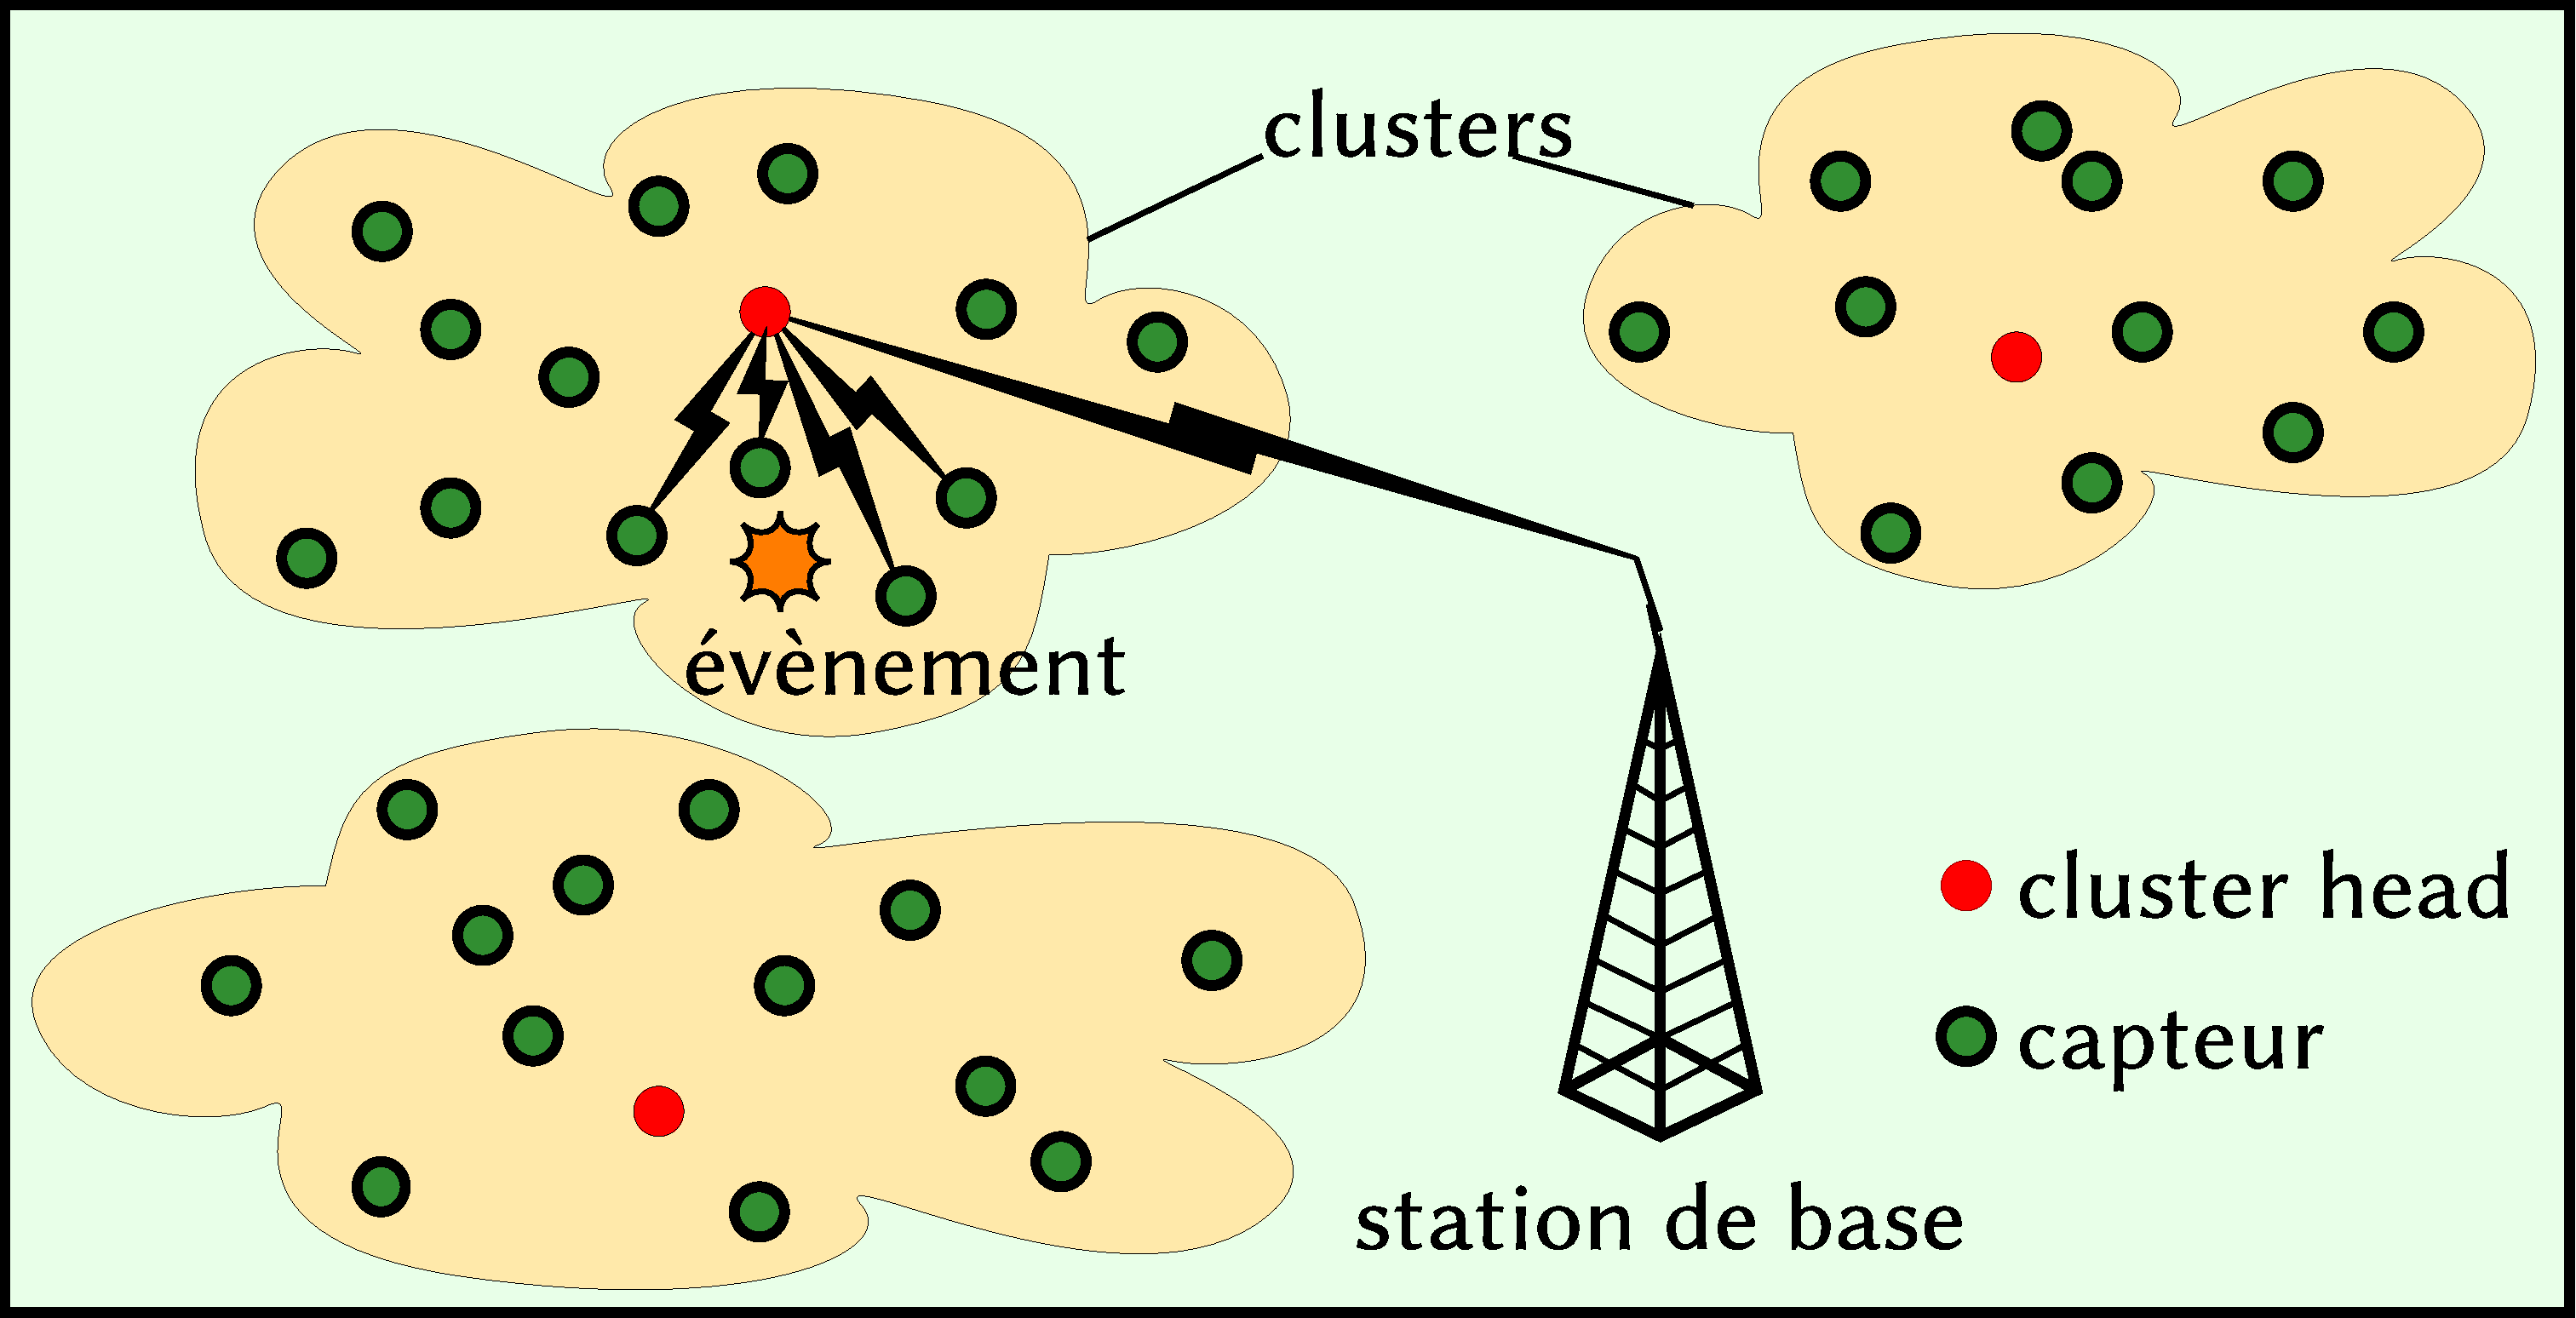
\includegraphics[width=0.8\linewidth]{\chapterfig/WSN.pdf}
    \caption{Schéma d'un \rc clusterisé}\label{st:fig:wsn}
\end{figure}

L'appel à un algorithme de «\idx{clusterisation}» a pour effet de limiter les émissions à «longue portée» (relativement aux communications intra-clusters) aux \chs seulement.
Or les communications sur de plus grandes distances se traduisent par une plus grande consommation en énergie (puisqu'une plus grande puissance d'émission est nécessaire).
Les capteurs normaux (non \chs) n'ont pas à atteindre directement des nœuds situés en dehors de leur cluster; ils économisent d'autant en énergie.
De plus, les \chs sont idéalement placés pour réaliser des opérations d'\idx{agrégation} voire de \idx{compression} sur les paquets qu'ils reçoivent, afin de limiter encore le volume des retransmissions couteuses en énergie.

À part les économies substantielles en énergie, la \idx{clusterisation} d'un réseau présente plusieurs autres avantages:
\begin{itemize}
    \item elle permet de déployer une gestion «centralisée» d'un cluster, puisque le \ch est à même d'appliquer un algorithme tenant compte de tous les capteurs de son groupe. Pour autant, la topologie décentralisée de l'ensemble du réseau n'est pas sacrifiée, car les clusters sont indépendants de la \sdb, qui n'intervient pas dans leur fonctionnement interne;
    \item elle permet de gagner en \idx{extensibilité}, puisqu'il est aisé de rajouter des clusters au réseau, voire peu contraignant de rajouter des nœuds dans un cluster donné. L'évolution du réseau est ainsi plus simple à assurer que s'il fallait modifier un algorithme distribué pour prendre en compte l'intégration de nouveaux capteurs.
\end{itemize}
%2}}}

        \subsubsection{Clusterisation hiérarchique\index{clusterisation!clusterisation hiérarchique}}
%{{{2
Une fois le \rc divisé en clusters, rien n'empêche de considérer les clusters un à un et de leur appliquer à nouveau un algorithme de \idx{clusterisation}, de façon à établir des sous-ensembles dans chaque cluster.
Et ainsi de suite, de façon récursive, jusqu'à atteindre le degré de hiérarchie désiré.
L'intérêt de cette méthode est de créer une partition hiérarchique\index{clusterisation!clusterisation hiérarchique} dans le réseau, permettant un meilleur contrôle des sous-ensembles de capteurs.
Par ailleurs, les clusters situés tout en bas dans la hiérarchie constituée seront de petite taille.
Les communications intra-clusters seront donc peu consommatrices en énergie.

Pour pouvoir distinguer plus facilement le niveau de hiérarchie auquel nous nous plaçons, nous désignerons par la suite sous le terme \textit{$k$-cluster} ($0 \leq k \leq$~nombre de capteurs) un sous-ensemble obtenu après $k$ applications de l'algorithme de \idx{clusterisation}.
En suivant cette convention, l'unique $0$-cluster est alors le réseau tout entier.
Lorsque nous parlons simplement de \textit{clusters}, il faudra comprendre $1$-clusters; autrement dit, des clusters issus d'une partition simple, sans degré supplémentaire de hiérarchie.

De même, on désignera par $k$-\ch (ou bien par $k$-\CH) les \chs de chacun des $k$-clusters du réseau.
Le rôle de $0$-\CH pourra alors être attribué à la \sdb.
Chaque $k$-\CH reçoit des données (provenant soit de nœuds normaux si $k$ est le dernier degré de la hiérarchie constituée, soit de ($k+1$)-\CH), les agrège\index{agrégation} et les transmet au ($k-1$)-\CH auquel il est rattaché.
%2}}}

        \subsubsection{Un exemple: fonctionnement de l'algorithme \leach}\label{st:subsubsec:leach}
%{{{2
L'un des algorithmes de \idx{clusterisation} les plus simples et les plus couramment employés dans les \rcsfs est l'algorithme \leach (\textit{Low Energy Adaptive Clustering Hierarchy}, \cad «hiérarchie de clusterisation adaptative à faible énergie» en anglais)~\cite{HCB00}.
Il s'agit d'un algorithme dynamique (il effectue de nouvelles clusterisations\index{clusterisation} du réseau régulièrement dans le temps) qui, par la formation de clusters, met en place une solution de \idx{routage} simple mais efficace des paquets dans le réseau.

Voici le fonctionnement détaillé de cet algorithme.
Soit $P$ le pourcentage moyen de \CHs désirés parmi le total des nœuds dans le réseau à un instant quelconque $t$.
\leach est découpé (dans la durée) en cycles, chacun constitué de $\frac{1}{P}$~rondes.
Chaque ronde $r$ est organisée de la façon suivante:
\begin{enumerate}
    \item Chaque nœud du réseau à partitionner calcule une valeur de seuil $S(i)$:
        \[
            S(i) = \left\{
            \begin{array}{cl}
                \displaystyle \frac{P}{1-P\cdot\left(r\mbox{ mod }\frac{1}{P}\right)} & \mbox{si }i\mbox{ n'a pas encore été \CH}\\
                                                                     0 & \mbox{si }i\mbox{ a déjà été \CH}
            \end{array}
            \right.
        \]
        Chaque nœud choisit un nombre pseudo-aléatoire $0 \le x_{i}\le 1$.
        Si $x_{i} \le S(i)$, alors $i$ s'auto-désigne comme \CH pour la ronde en cours.
        Il est à noter que le calcul de $S(i)$ est réalisé de telle façon que chaque nœud devienne \ch une fois et une fois seulement au cours de chaque cycle de $\frac{1}{P}$~rondes: le taux de probabilité d'auto-désignation\index{selection@sélection!auto-élection} $S(i)$ est égal à $1$ lorsque la fin du cycle est atteinte (autrement dit, lorsque $r = \frac{1}{P}-1$).
    \item Les \CHs auto-désignés informent leurs nœuds voisins de leur changement de statut à l'aide de messages en diffusion générale (\textit{broadcast}).
        Tous ces messages sont envoyés en utilisant la même puissance de transmission (valeur fixe et prédéterminée lors de l'implémentation).
        Pour limiter les collisions\index{collision}, il est fait usage sur la couche \mac de la méthode \textit{Carrier Sense Multiple Access} (\csma).
    \item Les autres nœuds, qui ne se sont pas désignés en tant que \chs pour la ronde en cours, choisissent de se joindre au cluster du \CH dont ils perçoivent le signal avec l'intensité la plus élevée, \cad le \CH le plus proche en termes de puissance du signal électromagnétique.
        Chaque nœud prévient le \ch qu'il décide de rejoindre en lui envoyant un message.
        La méthode \csma est là encore appliquée.
    \item Au vu des réponses reçues, chaque \ch calcule un «ordre de transmission» pour les nœuds qui l'ont rejoint.
        Il annonce alors à chacun de ces nœuds l'instant auquel le nœud doit lui transmettre ses données.
        Dans chaque cluster, les nœuds s'adresseront donc à leur \ch à tour de rôle, selon l'ordre déterminé par le \CH, ce qui revient à utiliser la méthode appelée \textit{Time Division Multiple Access} (\tdma).
    \item La phase de collecte des données peut débuter.
        Les \chs restent en écoute et reçoivent les données des autres capteurs de leur cluster.
        Les capteurs «normaux» effectuent leur mission (ils réalisent des mesures sur leur environnement), et envoient leurs résultats au \ch lorsque c'est à leur tour de le faire.
        Quand ce n'est pas à leur tour de communiquer, ces nœuds mettent leur équipement radio en veille afin d'économiser leur énergie.
        Les collisions\index{collision} entre les transmissions des nœuds de différents clusters sont évitées grâce à la méthode appelée \textit{Code Division Multiple Access} (\cdma).
    \item Au fur et à mesure qu'ils reçoivent les données, les \chs agrègent\index{agrégation}, et éventuellement compressent\index{compression} ces dernières.
        Ils les envoient ensuite à la \sdb, soit au cours d'une unique transmission directe, soit en faisant relayer les paquets par d'autres \chs.
    \item Les étapes~5 et~6 sont répétées jusqu'à la fin de la ronde.
\end{enumerate}

Quelques remarques sont à énoncer.
Tout d'abord: pour un cluster donné, il est alors possible de réitérer l'application de l'algorithme \leach, afin de créer une nouvelle partition au sein même d'un cluster.
Et ainsi de suite par récursivité, jusqu'à obtenir le degré de hiérarchie\index{clusterisation!clusterisation hiérarchique} désiré dans le réseau.
Nous appellerons $k$-\leach cet algorithme appliqué de façon à créer $k$ degrés hiérarchiques.

Second point: l'un des aspects importants de \leach est que lors de la première étape, chaque nœud choisi d'être, ou non, un \ch pour la ronde en cours.
Ce choix est basé uniquement sur la valeur de seuil calculée, et sur le nombre pseudo-aléatoire généré; à aucun moment un nœud ne fait intervenir dans sa décision le comportement de ses voisins.
En conséquence, le pourcentage $P$ de \chs désirés dans le réseau n'est qu'une valeur moyenne sur l'ensemble des rondes de chaque cycle.
Par ailleurs, la répartition géographique (au regard de la puissance de transmission nécessaire) idéale des \chs n'est en rien assurée.
Au contraire, il est même probable d'obtenir, pour certaines rondes, une concentration importante de \chs dans une zone restreinte du réseau, tandis que d'autres régions seront mal couvertes.
Il n'y a pas grand-chose à faire dans ce cas, sinon espérer que la prochaine ronde produira une distribution des \CHs plus favorable.
Si toutefois un nœud ne parvient à capter les messages d'aucun \CH, il se déclare généralement lui-même \ch.
%2}}}

        \subsubsection{De nombreux algorithmes de \idx{clusterisation}}
%{{{2
De nombreux algorithmes de \idx{clusterisation} de données existent.
Plusieurs d'entre eux sont même spécifiquement adaptés aux \rcsfs.
C'est le cas de \leach qui prend place, comme évoqué plus haut, parmi les plus fréquemment utilisés, à tel point qu'il en existe de nombreuses variantes.
Par exemple, il est possible d'étendre l'algorithme pour prendre en compte l'énergie restante dont dispose chaque nœud lors de l'\election des \CH.
Cette énergie résiduelle intervient alors en temps que paramètre supplémentaire lors du calcul de la valeur de seuil $S(i)$~\cite{HHT02}.
D'autres travaux sont basés sur \leach, que ce soit pour améliorer ses performances~\cite{RR13,CJ14} ou bien sa \secu~\cite{OFVWBDL07}.

Mais on trouve également de nombreux autres protocoles~\cite{AY07,DQWH13}.
Certains d'entre eux prennent en compte deux à trois paramètres, comme l'énergie résiduelle des nœuds, leur distance aux \chs potentiels et/ou le nombre de voisins de ces derniers: c'est le cas du protocole \heed~\cite{YF04}, assez souvent utilisé, ou du protocole MPC~\cite{KTAA12}, plus récent et moins répandu, se basant sur les k-moyennes.
Un quatrième élément, la \idx{confiance} portée au nœud, est même utilisé parfois pour réaliser une sélection plus sure des \CH~\cite{KMSL09}.

Certains protocoles ont des buts plus précis, comme \ffuca~\cite{FL11,FMMMI12} qui repose sur l'exploitation de propriétés ultramétriques dans le réseau afin de créer une répartition «idéale» des nœuds dans les clusters en fonction de leur distance aux \CH; ou bien comme VSR~\cite{TV08}, créé à l'intention des \manet, qui à l'aide d'une structure virtuelle détermine un \idx{routage} proactif pour l'intérieur des clusters (où les nœuds émettent au \ch en plusieurs sauts) et à la demande sur l'épine dorsale du réseau qui relie entre eux les \CH\,\footnote{Pour conserver la lisibilité du paragraphe, le développement des sigles HEED, FFUCA, MPC et VSR n'est pas donné ici. Il est néanmoins disponible \hyperref[sigles]{en fin d'ouvrage}.}.
\nomenclature{LEACH}{\textit{Low-Energy Adaptive Clustering Hierarchy}}
\nomenclature{HEED}{\textit{Hybrid, Energy-Efficient Distributed clustering}}
\nomenclature{FFUCA}{\textit{Fast and Flexible Unsupervised Clustering Algorithm }}
\nomenclature{MPC}{\textit{Multiple Parameter based Clustering}}
\nomenclature{VSR}{\textit{Virtual Struture Routing protocol}}
%2}}}
%1}}}

    \subsection{Déploiement autonome, \idx{mobilité}}
%{{{1
%{{{2
Les capteurs doivent être à même d'établir seuls une organisation autonome du réseau: ils comptent sur les protocoles inscrits dans leur mémoire, mais non sur une intervention externe (de l'administrateur par exemple).
L'organisation présente un défi en soi~\cite{TV08}, auquel les nombreux protocoles de découvertes des voisins et les algorithmes de \idx{routage} proposés au fil des ans apportent autant de réponses~\cite{DQWH13}.
Par ailleurs, ces protocoles sont tenus de gérer le départ ou l'arrivée de nouveaux nœuds dans le réseau.
C'est ce que l'on appelle l'\idx{extensibilité} du réseau (ou bien son évolutivité, ou encore sa scalabilité; \textit{scalability} est le terme anglais dénotant ce concept).

Qui plus est, il n'y a pas que le \idx{routage}, mais l'intégralité de la chaine des opérations à réaliser qui doit être mise en place de façon autonome: la collecte de données en fait ainsi partie~\cite{ZWPT10}.
Un autre paramètre à gérer parfois est la \idx{mobilité} des nœuds.
Cette \idx{mobilité} est une capacité propre aux \manet (\textit{Mobile Ad hoc Networks}, «réseaux ad hoc mobiles»).
Comme leur nom l'indique, il s'agit de \wanet dont les nœuds sont mobiles\index{mobilité}.
Lorsque ces nœuds sont (portés par) des véhicules, on parle même de \vanet (\textit{Vehicular Ad hoc Networks}, «réseaux ad hoc véhiculaires»).
Ces réseaux ont leurs propres problématiques~\cite{DYK12}, qui sont souvent assez proches de celles des \rcsfs.
Certaines solutions développées pour les \manet, des mécanismes de \secu par exemple, peuvent tout à fait être réutilisés dans les \rcs~\cite{BMS13}.

Mais revenons à la \idx{mobilité} en elle-même: elle n'est pas systématique dans les \rcsfs, dont les nœuds sont la plupart du temps statiques ou quasiment statiques.
Il arrive néanmoins que des réseaux soit constitués, en intégralité ou bien en partie, par des capteurs mobiles\index{mobilité}.
Le fait de se retrouver dans un environnement où les distances et les vitesses évoluent continuellement rend accessibles de nouvelles applications, mais vient bien sûr compliquer le \idx{routage}, la collecte des données, et même la gestion de la \idx{mobilité} des nœuds (s'ils n'ont pas de pilotes humains par exemple, il faut éviter les collisions~\cite{E-ZCGGK12})\index{collision}.
Dans le cas de \rcs comportant des nœuds mobiles\index{mobilité}, le modèle du réseau se verra en général rattaché aux \manet et, bien que ne bénéficiant pas forcément des mêmes ressources, ce sont les mêmes algorithmes de \idx{routage} qui vont être utilisés pour assurer l'acheminement des paquets de bout en bout.
Nous reviendrons plus loin sur des solutions reposant sur un nombre restreint de nœuds mobiles\index{mobilité} se déplaçant au sein d'un réseau de capteurs fixes pour réaliser différentes opérations sur les appareils (collecte de données, diffusion d'information, réinitialisation de la configuration d'origine, \etc)~\cite{HR13}.
\nomenclature{MANET}{\textit{Mobile Ad hoc NETworks}}
\nomenclature{VANET}{\textit{Vehicular Ad hoc NETworks}}
%2}}}
%1}}}

    \subsection{Sécurité\index{securité@sécurité}, \idx{sureté} et \resilience}
%{{{1
        \subsubsection{Sureté\index{sureté}, \resilience}
%{{{2
Comme évoqué précédemment, une fois déployés, les \rcs doivent s'organiser et fonctionner seuls, sans intervention humaine.
Pour autant, ils ne sont pas à l'abri des erreurs ni des pannes.
L'idéal est donc de pouvoir assurer un certain degré de \idx{sureté} et de \resilience au réseau.

La \idx{sureté} d'un système est sa capacité à fonctionner sans erreurs, \cad sans dysfonctionnement dus à une mauvaise conception ou à une mauvaise implémentation des architectures matérielle et logicielle.
Elle est en principe apportée soit par des tests en amont du déploiement, soit par une \idx{modélisation} formelle (ou semi-formelle) du système, qui permet d'en évaluer certaines propriétés et de déduire, en fin de compte, si le système mis en place respecte ou non les spécifications établies.

Les tests et simulations sont récurrents dans la quasi-totalité des travaux de la littérature.
Ils consistent à implémenter le dispositif étudié, physiquement ou virtuellement, pour étudier son évolution au cours d'une exécution «classique» ou bien soumise à des conditions d'expérimentation particulières.
Certains travaux ont même pour objet des tests comparatifs sur différentes architectures matérielles de capteurs~\cite{PLP06}, ou encore recensent les différents systèmes de simulation permettant d'expérimenter sur les réseaux de capteurs~\cite{AAAHN12}.

Pour la vérification basée sur des méthodes formelles, des outils tels que le \modelchecking peuvent par exemple être appliqués sur le modèle établi.
Le \modelchecking est une technique pouvant être utilisée sur des systèmes concurrents à états finis, et qui permet d'extraire automatiquement certaines propriétés sur les performances ou la \idx{sureté} du modèle puis de s'assurer qu'elles sont respectées dans le réseau à tout instant.
Si le système ne fonctionne pas comme prévu, l'outil permet parfois d'obtenir une trace qui vient faciliter la localisation de la source de l'erreur.
Contrairement aux tests et aux simulations, les résultats obtenus à l'aide du \modelchecking ne varient pas entre deux instances.
Encore mieux: la spécification formelle du système permet de vérifier les propriétés sur tous les cas possibles d'exécution déterminés par les spécifications du modèle, tandis que des simulations ne permettent de remonter que certaines erreurs détectées (sans assurance de les avoir trouvées toutes).
Le \modelchecking est utilisé régulièrement dans les réseaux sans fils, que ce soit pour valider la conception de protocoles de \idx{routage} comme pour la vérification de propriétés de \idx{sureté} concernant les risques de collisions\index{collision} au sein d'un groupe de véhicules~\cite{E-ZCGGK12}.
%2}}}

        \subsubsection{Résilience\index{resil@résilience}}
%{{{2
La \resilience d'un système est la capacité de ce système à outrepasser et éventuellement à corriger les erreurs susceptibles de survenir.
Autrement dit, un système résilient est capable de poursuivre son fonctionnement avec toujours autant d'efficacité ou presque, même si des pannes matérielles, des erreurs logicielles ou d'autres types d'incidents viennent perturber le système.
Assurer la \resilience revient donc à anticiper, à prévoir des «plans de secours», des mécanismes de correction et de réparation automatiques.

Concrètement, dans un \rcsfs, elle met en jeu des principes comme la \idx{redondance} des données stockées et envoyées, ou des routes\index{routage!route} de retransmission~\cite{SP10}; elle s'établit sur l'usage de protocoles capables de se mettre à jour lorsque des nœuds disparaissent (épuisement supposé) ou apparaissent (nouveaux arrivants) dans le réseau, de mécanismes de correction d'erreurs…\index{correction d'erreur}
La \resilience matérielle passe le plus souvent par la \idx{redondance} des composants, mais n'est que rarement mise en place, pour des raisons de couts, dans les \rcs.
On préféra en général utiliser quelques capteurs en plus par rapport à la quantité strictement nécessaire pour assurer le service, sans avoir à augmenter le prix de \emph{tous} les capteurs.

La \idx{sureté} et la \resilience des réseaux ne sont pas des problématiques de \secu (car aucune attaque volontaire ne rentre en compte), mais il s'agit de problématiques assez proches de la \idx{disponibilité} des réseaux (définie au \chapref{ea}, \ssref{ea:def:dispo}).
%2}}}

        \subsubsection{Sécurité\index{securité@sécurité}}
%{{{2
En raison de leurs faibles capacités, conjuguées aux domaines critiques dans lesquels ils interviennent parfois, les capteurs peuvent présenter des cibles de choix pour un attaquant.
Les algorithmes et mécanismes classiques utilisés en \idx{cryptographie} afin d'assurer la \idx{confidentialité} ou l'\idx{authentification} des données sont souvent très exigeants en ressources (en termes de calculs notamment, et donc de consommation énergétique).
Il a fallu adapter ces mécanismes aux capteurs.

D'autres attaques peuvent être menées, non plus pour intercepter des données, mais dans le but de perturber le bon fonctionnement du réseau.
Ce sont les attaques dites par \textit{\dds}.
Un attaquant, par le biais d'un nœud compromis par exemple, peut ainsi chercher à détourner des flux de données au sein du réseau, à empêcher des paquets de parvenir à destination (en les supprimant), à maximiser le débit du nœud compromis au détriment de celui des autres nœuds, à saturer le canal de transmission pour empêcher les nœuds légitimes de l'utiliser, ou encore à pousser les autres capteurs à l'épuisement de leurs réserves en énergie, \etc.
Pour rappel, l'objectif des travaux présentés dans cet ouvrage consiste à proposer, modéliser et tester une solution permettant de détecter, puis de réagir aux attaques de ce type, tout en assurant une consommation minimale en ressources pour les capteurs du réseau.

\paragraph{}
Bien que le thème de la \secu des \rcsfs, notamment sur le sujet des attaques de type «\dds» ainsi que des contre-mesures appropriées, ait tout à fait sa place dans ce chapitre, il s'agit d'un élément central pour les travaux de cet ouvrage, et il est développé avec beaucoup plus de précisions que les problématiques précédentes.
Aussi a-t-il été choisi de lui attribuer un chapitre spécifique: les pages qui suivent abordent la question de la \secu avec bien plus de détails que jusqu'à présent.
%2}}}
%1}}}
